\section{Hardness of PCC in the presence of an oracle}
\begin{theorem}
Given that the Exponential Time Hypothesis (ETH) holds then any algorithm for the Promise Correlation Clustering problem  that runs in polynomial time makes $\Omega(|X|)$ same-cluster queries for all $M \ge 3$ and for $\alpha = 0$ and $\beta = \frac{1}{2}$. 
\end{theorem}

\noindent The exponential time hypothesis says that any solver for $3$-SAT runs in $2^{o(m)}$ time (where $m$ is the number of clauses in the $3$-SAT formula). We use a reduction from $3$-SAT to 3DM to X3C to show that the exact cover by 3-sets (X3C) problem also can't be solved in $2^{o(m)}$ time (if ETH holds). Then, using the reduction from the previous section implies that PCC also can't be solved in $2^{o(n)}$ time. Thus, any query based algorithm for PCC needs to make atleast $\Omega(n)$ queries where $n = |X|$ is the number of vertices in the graph. 

\begin{definition}[3-SAT].\\
Input: A boolean formulae $\phi$ in 3CNF with $n$ literals and $m$ clauses. Each clause has exactly three literals. \\
Output: YES if $\phi$ is satisfiable, NO otherwise. 
\end{definition}

\noindent\textbf{Exponential Time Hypothesis}\\
There does not exist an algorithm which decides 3-SAT  and runs in $2^{o(m)}$ time.

\begin{definition}[3DM].\\
Input: Sets $W, X$ and $Y$ and a set of matches $M \subseteq W \times X \times Y$ of size $m$.  \\
Output: YES if there exists $M' \subseteq M$ such that each element of $W, X, Y$ appears exactly once in $M'$. NO otherwise. 
\end{definition}

\noindent To prove that (X3C) is NP-Hard, the standard We will reduce 3-SAT to 3-dimensional matching problem. 3DM is already known to be NP-Hard. However, the standard reduction of 3-SAT to 3DM constructs a set with $|M| \in \Theta(m^2 n^2)$. Hence, using the standard reduction, the exponential time hypothesis would imply there does not exist an algorithm for 3DM which runs in $\Omega(m^\frac{1}{4})$. Our reduction is based on the standard reduction. However, we make some clever optimizations especially in the way we encode the clauses. This helps us improve the lower bound to $\Omega(m)$.

\begin{figure}[!ht]
	\centering
	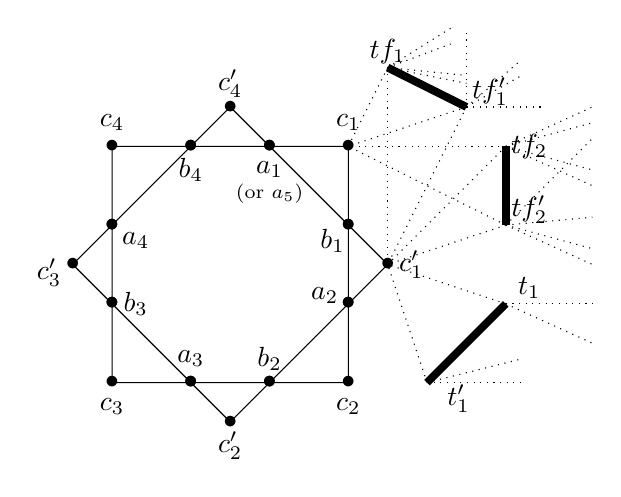
\begin{tikzpicture}
	  \draw (0,0) node {$\bullet$} -- (1,0) node{$\bullet$} -- (0.5,0.5) node{$\bullet$} -- cycle;
	  \draw (1,0) node{$\bullet$} -- (2,0) node{$\bullet$}
  -- (2,-1) node{$\bullet$} -- cycle;
	  \draw (2,-1) node{$\bullet$} -- (2,-2) node{$\bullet$} -- (2.5,-1.5) node{$\bullet$} -- cycle;
	  \draw (2,-2) node{$\bullet$} -- (1,-3) node{$\bullet$} -- (2,-3) node{$\bullet$} -- cycle;
	  \draw (0,-3) node{$\bullet$} -- (1,-3) node{$\bullet$} -- (0.5,-3.5) node{$\bullet$} -- cycle;
	  \draw (0,-3) node{$\bullet$} -- (-1,-2) node{$\bullet$} -- (-1,-3) node{$\bullet$} -- cycle;
	  \draw (-1,-2) node{$\bullet$} -- (-1,-1) node{$\bullet$} -- (-1.5,-1.5) node{$\bullet$} -- cycle;
	  \draw (0,0) node{$\bullet$} -- (-1,-1) node{$\bullet$} -- (-1,0) node{$\bullet$} -- cycle;
	
	 \node  at (0.0,-0.3) {$b_4$};
	 \node  at (1.0,-0.3) {$a_1$};
	 \node  at (1.0,-0.6) {\scriptsize{(or $a_5$)}};
	 \node  at (2.0,0.3) {$c_1$};
	 \node  at (1.8,-1.2) {$b_1$};
	 \node  at (1.7,-1.9) {$a_2$};
	 \node  at (2.8,-1.5) {$c_1'$};
	 \node  at (2.0,-3.3) {$c_2$};
	 \node  at (1.0,-2.7) {$b_2$};
	 \node  at (0.0,-2.7) {$a_3$};
	 \node  at (0.5,-3.8) {$c_2'$};
	 \node  at (-1.0,-3.3) {$c_3$};
	 \node  at (-0.7,-2.0) {$b_3$};
	 \node  at (-0.7,-1.2) {$a_4$};
	 \node  at (-1.8,-1.6) {$c_3'$};
	 \node  at (-1.0,0.3) {$c_4$};
	 \node  at (0.5,0.8) {$c_4'$};
	 
	 \node  at (2.5,1.2) {$tf_1$};
	 \node  at (3.8,0.7) {$tf_1'$};
	 \node  at (4.3,0.0) {$tf_2$};
	 \node  at (4.3,-0.8) {$tf_2'$};
	 \node  at (4.3,-1.8) {$t_1$};
	 \node  at (3.4,-3.2) {$t_1'$};

	 \draw [line width=1mm] (4,0) -- (4,-1);
	 %\node  at (4.3,-0.5) {$\gamma_i$};
	 \draw [line width=1mm] (2.5,1) -- (3.5,0.5);
	 %\node  at (3.2,0.9) {$\beta_i$};
	 \draw [line width=1mm] (4,-2) -- (3,-3);
  	 %\node  at (3.8,-2.6) {$\alpha_i$};
	 
  	\draw[dotted](4, 0) -- (2, 0);
  	\draw[dotted](4, -1) -- (2, 0);
  	\draw[dotted](4, 0) -- (2.5, -1.5);
  	\draw[dotted](4, -1) -- (2.5, -1.5);
  	\draw[dotted](4, 0) -- (5.1, 0.5);
  	\draw[dotted](4, 0) -- (5.1, 0.3);
  	\draw[dotted](4, 0) -- (5.1, -0.5);
  	\draw[dotted](4, 0) -- (5.1, -0.3);
  	\draw[dotted](4, -1) -- (5.1, 0.1);
  	\draw[dotted](4, -1) -- (5.1, -0.9);
  	\draw[dotted](4, -1) -- (5.1, -1.5);
  	\draw[dotted](4, -1) -- (5.1, -1.3);

  	\draw[dotted](2.5, 1) -- (2, 0);
  	\draw[dotted](3.5, 0.5) -- (2, 0);
  	\draw[dotted](2.5, 1) -- (2.5, -1.5);
  	\draw[dotted](3.5, 0.5) -- (2.5, -1.5);
  	\draw[dotted](2.5, 1) -- (3.3, 1.5);
  	\draw[dotted](2.5, 1) -- (3.3, 1.3);
  	\draw[dotted](2.5, 1) -- (3.5, 0.9);
  	\draw[dotted](2.5, 1) -- (3.5, 0.8);
  	\draw[dotted](3.5, 0.5) -- (4.2, 1.1);
  	\draw[dotted](3.5, 0.5) -- (4.2, 0.9);
  	\draw[dotted](3.5, 0.5) -- (3.5, 1.5);
  	\draw[dotted](3.5, 0.5) -- (4.5, 0.5);

  	\draw[dotted](4, -2) -- (2.5, -1.5);
  	\draw[dotted](3, -3) -- (2.5, -1.5);
  	\draw[dotted](4, -2) -- (5.1, -2);
  	\draw[dotted](4, -2) -- (5.1, -2.5);
  	\draw[dotted](3, -3) -- (4.2, -3);
  	\draw[dotted](3, -3) -- (4.2, -2.7);
  	\end{tikzpicture}
  	\caption{Part of graph $G$ constructed for the literal $x_1$. The figure is an illustration for when $x_1$ is part of four different clauses. The triangles (or hyper-edge) $(a_i, b_i, c_i)$ capture the case when $x_1$ is true and the other triangle $(b_i, c_i', a_{i+1})$ captures the case when $x_1$ is false. Assuming that a clause $C_j = \{x_1, x_2, x_3\}$, the hyper-edges containing $tf_i, tf_i'$ and $t_1, t_1'$ capture different settings. The hyper-edges containing $t_1, t_1'$ ensure that atleast one of the literals in the clause is true. The other two ensure that two variables can take either true or false values.}
\label{fig:3DMQueries}
\end{figure}

Our gadget is described in Fig. \ref{fig:3DMQueries}. For each literal $x_i$, let $m_i$ be the number of clauses in which the the literal is present. We construct a ``truth-setting" component containing $2m_i$ hyper-edges (or triangles). We add the following hyper-edges to $M$.
\begin{align*}
  &\{(a_k[i], b_k[i], c_k[i]): 1 \le k \le m_i\} \cup \{(a_{k+1}[i], b_k[i], c_k'[i]): 1 \le k \le m_i\}
\end{align*}
Note that one of $(a_k, b_k, c_k)$ or $(a_{k+1}, b_k, c_k')$ have to be selected in a matching $M'$. If the former is selected that corresponds to the variable $x_i$ being assigned true, the latter corresponds to false. This part is the same as the standard construction. 

For every clause $C_j = \{x_1, x_2, x_3\}$ we add three types of hyper-edges.  The first type ensures that atleast one of the literals is true. 
$$\{(c_k[i], t_1[j], t_1'[j]): x_i' \in C_j\} \cup \{(c_k'[i], t_1[j], t_1'[j]): x_i \in C_j\}$$ 
The other two types of hyper-edges (conected to the $tf_i$'s) say that two of the literals can be either true or false. Hence, we connect them to both $c_k$ and $c_k'$
\begin{align*}
  &\{(c_k[i], tf_1[j], tf_1'[j]): x_i' \text{ or }x_i\in C_j\} \cup \{(c_k[i], tf_2[j], tf_2'[j]): x_i \text{ or }x_i' \in C_j\}\\
  &\cup \{(c_k'[i], tf_1[j], tf_1'[j]): x_i' \text{ or }x_i\in C_j\} \cup \{(c_k'[i], tf_2[j], tf_2'[j]): x_i \text{ or }x_i' \in C_j\}
\end{align*}
Note that in the construction $k$ refers to the index of the clause $C_j$ in the truth-setting component corresponding to the literal $x_i$. Using the above construction, we get that
\begin{align*}
  & W = \{c_k[i], c_k'[i]\}\\
  & X = \{a_k[i]\} \cup \{t_1[j], tf_1[j], tf_2[j]\}\\
  & Y = \{b_k[i]\} \cup \{t_1'[j], tf_1'[j], tf_2'[j]\}
\end{align*} 
Hence, we see that $|W| = 2\sum_i m_i = 6m$. Now, $|X| = |Y| = \sum_i m_i + 3m = 6m$. And, we have that $|M| = 2\sum_i m_i + 15m = 21m$. Thus, we see that this construction is linear in the number of clauses. 

Now, if the 3-SAT formula $\phi$ is satisfiable then there exists a matching $M'$ for the 3DM problem. If a variable $x_i = T$ in the assignment then add $(c_k[i], a_k[i], b_k[i])$ to $M'$ else add $(c_k'[i], a_{k+1}[i], b_k[i])$. For every clause $C_j$, let $x_i$ (or $x_i'$) be the variable which is set to true in that clause. Add $(c_k'[i], t_1[j], t_1'[j])$  (or $(c_k[i], t_1[j], t_1'[j])$) to $M'$. For the remaining two clauses, add the hyper-edges containing $tf_1[j]$ and $tf_2[j]$ depending upon their assignments. Clearly, $M'$ is a matching. 

Now, the proof for the other direction is similar. If there exists a matching, then one of $(a_k, b_k, c_k)$ or $(a_{k+1}, b_k, c_k')$ have to be selected in a matching $M'$. This defines a truth assignment of the variables. Now, the construction of the clause hyper-edges ensures that every clause is satisfiable.

\begin{theorem}
If the exponential time hypothesis holds then there does not exist an algorithm which decides the three dimensional matching problem 3DM and runs in time $2^{o(m)}$.
\end{theorem}

\begin{corollary}
\label{cor:X3CLowerBound}
If the exponential time hypothesis holds then there does not exist an algorithm which decides exact cover by 3-sets problem (X3C) and runs in time $2^{o(m)}$.
\end{corollary}

Hence, from the discussion in this section, we know that X3C is not only NP-Hard but the running time is lower bounded by $\Omega(2^m)$. Now, using the same reduction of X3C to PCC as before, gives the same lower bound on the running time of PCC. Using this, we can now lower bound the number of queries required by PCC.

For the sake of contradiction, let us assume that there exists an algorithm which solves PCC in polynomial time by making $o(n)$ same-cluster queries ($n$ is the number of vertices). Then by simulating all possible answers for the oracle, we get a non-query algorithm which solves PCC in $2^{o(n)}$. However, combining Cor. \ref{cor:X3CLowerBound} with the reduction of X3C to PCC, we get that any algorithm that solves PCC takes $\Omega(2^n)$. Hence, no such query algorithm exists. 

\section{Locality Sensitive Hashing}
\label{section:A-LSH}
The technique of locality sensitive hashing was introduced by \cite{gionis1999similarity} to solve the problem of approximate nearest neighbour search. The LSH-based hashing schemes try to put similar points into the same bucket. Hence, to search for points which are `similar' to a given point $x \in X$, one only needs to search within the same hash bucket instead of searching within the whole set $X$. Next, we describe a generic hashing based algorithm. 

\begin{definition}[LSH \cite{charikar2002similarity}]
\label{defn:LSH}
Given a set $X$ and a similarity function $f:X \times X \rightarrow [0, 1]$. Given a class of hash functions $H = \{h_1, h_2, \ldots \}$. An LSH w.r.t $X$ and $f$ is a probability distribution over $H$ such that for each $x, y \in \mc X$, $$\underset{h \in H}{\mb P}\enspace [h(x) = h(y)] = f(x, y)$$
\end{definition}
\noindent Some common examples of an LSH schemes are minhash scheme w.r.t jaccard similarity measure \cite{broder2000min, broder1997resemblance}, simhash scheme w.r.t hamming similarity measure \cite{charikar2002similarity}. We describe a generic locality sensitive hashing procedure in Alg. \ref{alg:LSH}. Observe that, Alg. \ref{alg:LSH} outputs $s$ different partitions of $X$. Assume without loss of generality, that a point $x$ lies in the blocks $B_{11} \in P_1, B_{21} \in P_2, \ldots, B_{s1} \in P_s$. Now, to search for points $y$ which are similar to $x$, we only need to search within the blocks $B_{i1}$. We say that these points lie in the same `bucket' as $x$. We say that $b(x, y) = 1$ if and only if $x$ and $y$ lie together in the same block in atleast one of the partitions.

\begin{algorithm}
\caption{A generic LSH based hashing algorithm \cite{indyk1998approximate,charikar2002similarity}}
\label{alg:LSH}

\Indp\KwIn{A set $X$, a similarity function $f$, a class of hash functions $H$ over $X$, integers $r, s$ and a perfect hash function $p$ over the domain $\mb N^r$.}
\KwOut{Partitions $P_1, \ldots, P_s$ of the set $X$.}
\vspace{0.1in} Let $D$ be a distribution over $H$ which satisfies Defn. \ref{defn:LSH} and let $k = r s$.\\
Sample hash functions $h_1, \ldots, h_k$ iid using $D$.\\
 Group the hash functions into $s$ bands. Each band contains $r$ hash functions. \\
For all $x$ and $1\le i \le s$,  let $g_i(x) = (h_{(i-1)s + 1}(x), \ldots, h_{ir}(x))$. That is, $g_i(x)$ represents the $i^{th}$ signature of $x$. \\
For all $1 \le i \le s$, obtain partitions $P_i$ of $\mc X$. That is, $P_i = \{B_{i1}, \ldots, B_{im_i}\}$ where each $B_{ij} = \{x : p(g_i(x)) = b_{ij}\}$ for some $b_{ij}$.\\
Output $\{P_1, \ldots, P_s\}$.
\end{algorithm}



Hence, to search for points which are similar to $x$, we need to search over $y$ such that $b(x, y) = 1$. Our sampling procedure will sample pairs from the set $\mc Q := \{(x, y) : b(x, y) = 1\}$ (details in the next section). Hence, a requirement from the hashing scheme is that we should be able to construct the set $\mc Q$ in linear time. Thm. \ref{thm:hashTimeComplexity} shows that this is indeed the case. 

\begin{restatable}{thrm}{hashTimeComplexity}
\label{thm:hashTimeComplexity}
Given $X$, a similarity function $f$, a class of hash functions $H$, integers $r, s$ and perfect hash function $p$. Alg. \ref{alg:LSH} runs in $O(|X|rs \max_{ij}|B_{ij}|)$.
\end{restatable}
\begin{proof}
Let $n = |X|$. Sampling $k$ different hash function takes $rs$ time. Computing the signatures for all $x$ takes $nrs$ time. Obtaining the different partition takes $ns$ time. Now, computing $R_x$ for all $x$ takes time $t = \sum_{i = 1}^b \sum_{j=1}^{m_j} |B_{ij}|^2$. Now, we know that for all $i$, $\sum_{j=1}^{m_j} |B_{ij}| = n$. Hence, $\sum_{j=1}^{m_j} |B_{ij}|^2 \le \max_j B_{ij} \enspace \sum_{j=1}^{m_j} |B_{ij}| = n \max_j{B_{ij}}$. Hence, $t \le n s \max_{ij} |B_{ij}|$.  
\end{proof}

\noindent We see that the running time is dependent upon the block sizes. If the maximum block size is a constant then the hashing scheme runs in linear time. Even when the block sizes are bounded by $\log n$, then the scheme runs in $O(n \log n)$.  Next, we show that a if $d(x, y) \le \lambda$ then $(x, y) \in \mc Q$ with very high probability. Also, if $d(x, y) > O(2\lambda)$ then with high probability $(x, y) \not\in \mc Q$.   

\begin{restatable}{thrm}{similarInSame}
\label{thm:similarInSame}
Given a set $X$, a distance function $d: X \times X \rightarrow [0, 1]$, a class of hash functions $H$, threshold parameter $\lambda$ and a parameter $\delta$. Let the similarity function be $f(x, y) := 1 - d(x, y)$ and let $\mc A$ be a generic LSH based algorithm (Alg. \ref{alg:LSH}) which outputs partitions $P_1, \ldots, P_s$. Let $b(x, y) = 1$ iff $x, y$ are together in atleast one of these partitions. 
\noindent Choose $r, s$ such that $\frac{1}{2\lambda} < r < \frac{1}{-\ln(1-\lambda)} $ and $s =  \lceil 2.2\ln(\frac{1}{\delta})\rceil$. Define $\delta' := s\ln(1+\delta)$. Then for $(x, y) \in \mc X^2$
\begin{itemize}
	\item If $d(x, y) \le \lambda$ then 
	\begin{align*}
		& \underset{h \in H}{\mb P} \enspace[\enspace b(x, y) = 1 ] \enspace > \enspace 1 - \delta
	\end{align*}
	\item If $d(x, y) > 2\lambda\ln\big(1+\frac{1}{\delta}\big)$ then 
	\begin{align*}
		& \underset{h \in H}{\mb P} \enspace[\enspace b(x, y) = 1 ] \enspace < \enspace \delta'
	\end{align*}
\end{itemize}
\end{restatable}
\begin{proof}
Observe that
\begin{align*}
  & \mb P[b(x, y) = 0] = \mb P \enspace  [ \underset{i=1}{\cap^s} g_i(x) \neq g_i(y)] \\
  &=\prod_i\Big(1 - \prod_{j=1}^r \mb P[ h_{(i-1)r+j}(x) = h_{(i-1)r+j}(y)]\Big)\\
  & = \prod_{i=1}^s(1 - \prod_{j=1}^r f(x, y)) = (1-f(x, y)^r)^s
\end{align*}
Consider the case when $d(x, y) \le \lambda$. From the choice of $s$, we know that $s \ge 2.2\ln(1/\delta) \implies s \ge \frac{\ln(1/\delta)}{1-\ln(e-1)}\iff 1-\frac{1}{e} \le \delta^{1/s}$. From the choice of $r$, we know that $r < \frac{1}{-\ln(1-\lambda)} \iff r \ln(\frac{1}{1-\lambda}) < 1 \iff (1-\lambda)^r > \frac{1}{e}$.  Hence,   then we have that $\mb P[b(x, y) = 0]  = (1 - (1-d(x, y))^r)^s \le (1 - (1-\lambda)^r)^s < \delta$. This proves the first part of the theorem. 

For the second part, consider the case when $d(x, y) > \lambda'$ where $\lambda'$ is such that $\ln(1+1/\delta) = \frac{\lambda'}{2\lambda}$. 
\begin{flalign*}
  & \frac{1}{2\lambda} < r \iff \frac{\ln(1+1/\delta)}{\lambda'} < r. \enspace\text{Now, $\lambda' \le \ln\Big(\frac{1}{1-\lambda'}\Big)$. Hence, }&\\
  &\implies \frac{\ln(1+1/\delta)}{\ln(\frac{1}{1-\lambda'})} < r \iff r\ln(1-\lambda') < \ln(\frac{\delta}{1+\delta}) &\\
  &\iff 1-(1-\lambda')^r > e^{-\ln(1+\delta)} = e^{-\delta'/s} > (1-\delta')^{1/s}&\\
  &\implies \mb P[b(x, y) = 0] > (1-(1-\lambda')^r)^s > 1-\delta'&
\end{flalign*}
Now, the only thing that remains to be shown is that we can choose an integer $r$ satisfying the conditions of the theorem. Consider the function $f(x) = -\frac{1}{2x} - \frac{1}{\ln(1-x)}$. Using elementary analysis, we see that for $x \rightarrow 0, f(x) \rightarrow \infty$. Infact, for $x \le 0.32, f(x) > 1$. Hence, for $\lambda \le 0.32$, $r$ satisfying the conditions of the theorem exists.
\end{proof}

\section{Proofs of theorems and lemmas}
\begin{restatable}{lem}{weightedNegUniform}
\label{lemma:weightedNegUniform}
Given $X$ and a $C^*$-oracle. The procedure $\mc P_0$ samples a pair $(x, y)$ according to the distribution $P^-$.
\end{restatable}
\begin{proof}
Refer to Lemma 11 in \cite{kushagra2018semisupervised}.
\end{proof}

\begin{restatable}{lem}{negQueries}
\label{lemma:negQueries}Given set $X$ and a $C^*$-oracle. Let $X$ be $\gamma$-skewed. Let $q$ be the number of same-cluster queries made by $\mc P_0$ to the $C^*$-oracle. Then, $\mb E[q] \le \frac{1}{1-\gamma}$.
\end{restatable}
\begin{proof}
Refer to Lemma 12 in \cite{kushagra2018semisupervised}.
\end{proof}

\posDistribution*
\begin{proof}
Let $Q := \{(x, y): b(x, y) = 1\} = \{(x, y) \in B^2: B \in \mc B\}$. Let $K = \{(x, y): d(x, y) \le \lambda\}$, let $K_Q = K\cap Q$, let $K^+ := \{(x, y) \in K: C^*(x, y) = 1\}$ and finally let $K_Q^+ = \{(x, y) \in K_Q : C^*(x, y) = 1\}$. Note that the choice of $Q$ depends upon the hashing algorithm $\mc A$. However, after the pre-compute stage, the set $Q$ is fixed and the sampling procedure samples from the set $Q$. Our procedure works in four steps. 
\begin{enumerate}[noitemsep,label=\textbf{S.\arabic*}]
  \item $\mc P_1$ samples a point $(x, y)$ from the set $Q$ and induces a distribution $D_1$ on $Q$. 
  \begin{align*}
    &D_1(x, y) = \sum_{B \in a(x, y)} \frac{|B|^2}{\sum_{B' \in \mc B}|B'|^2}\frac{1}{|B|^2} = \frac{|a(x, y)|}{\sum_{B' \in \mc B}|B'|^2}
  \end{align*}
  \item Next, we reject the sampled point with some probability thereby inducing another distribution $D_2$ on $Q$. Now, $D_2(x, y)$ satisfies the following recurrence
  \begin{align*}
    &D_2(x, y) = D_1(x, y) \frac{1}{|a(x, y)|} \\
    &+ \Big(1-\sum_{(x', y') \in Q} D_1(x', y') \frac{1}{|a(x', y')|}\Big)D_2(x, y)
  \end{align*}
  The recurrence basically says that the probability that the pair $(x, y)$ is sampled is equal to the probability that it is sampled during the current round or nothing is sampled during the current round and then $(x, y)$ is sampled. Simplifying the above equation, we get that
   \begin{align*}
    &D_2(x, y) = \frac{\frac{1}{\sum_{B' \in \mc B}|B'|^2}}{\sum_{(x', y') \in Q}\frac{1}{\sum_{B' \in \mc B}|B'|^2}} = \frac{1}{|Q|}
  \end{align*}
  \item We reject the sampled point if $(x, y) \not\in K_Q$. In this step, we induce a distribution $D_3$ on $K_Q$. It is easy to see that
  \begin{align*}
    &D_3(x, y) = \frac{1}{|K_Q|}
  \end{align*}
  \item \label{item:D4} Next, we reject the sampled point if $(x, y) \not\in K_Q^+$. After this step, we induce a distribution $D_4$ on $K^+_Q$.
  \begin{align*}
    &T(x, y) := D_4(x, y) = \frac{1}{|K_Q^+|}
  \end{align*}
  Another observation, which will be useful later in the proof is that for any $(x, y) \in K^+$, $\mb P[(x, y) \in K_Q^+] > 1-\delta$ (Thm. \ref{thm:similarInSame}). Hence, using multiplicative chernoff's bounds we get that, $\mb P\big[|K_Q^+| > (1-\nu)|K^+|(1-\delta)\big] \ge 1- \exp\Big(\frac{-\nu^2 (1-\delta) |K^+|}{2}\Big)$ 
\end{enumerate}
Next, we will show that the distribution $T$ is an approximation of $P^+$. First, observe that $\mc X$ satisfies $\mu$-nazdeek property. Hence, we get that 
\begin{align*}
  &1 - \alpha \le \mb P[d(x, y) \le \lambda| C^*(x, y) = 1] = \frac{|K^+|}{|X^2_+|} \numberthis\label{eqn:KplusX2plus}
\end{align*}
Now, let $h$ be any labelling function over $\mc X^2$.
\begin{align*}
  &\underset{(x, y) \sim T}{\mb P} [C(x, y) = 0] = \frac{1}{|K_Q^+|}\sum_{(x, y) \in K^+_Q} \mb 1_{[C(x, y) = 0]}\\
  & \le \frac{1}{|K_Q^+|}\sum_{(x, y) \in X^+_2} \mb 1_{[C(x, y) = 0]}
\end{align*}
Now, with probability atleast $1- \exp(\frac{-\nu^2 (1-\delta) |K^+|}{2}) \ge 1 - \exp(\frac{-\nu^2 (1-\delta)(1-\nu) |X^2_+|}{2}) $ over the randomness in $\mc A$, we have that $|K_Q^+| > (1-\nu)(1-\delta)|K^+|$. Substituting this in the above equation gives
\begin{align*}
  &\underset{(x, y) \sim T}{\mb P} [C(x, y) = 0]  \le \frac{1}{(1-\nu)(1-\delta)|K^+|}\sum_{(x, y) \in X^2_+} \mb 1_{[C(x, y) = 0]}\\
  &\le \frac{1}{(1-\nu)(1-\delta)(1-\alpha)|X^2_+|}\sum_{(x, y) \in X^+_2} \mb 1_{[C(x, y) = 0]} \\
  &= \frac{\underset{(x, y) \sim P^+}{\mb P} [C(x, y) = 0]}{(1-\nu)(1-\delta)(1-\alpha)}
\end{align*}
Now for the other direction, we have that
\begin{align*}
  &\underset{(x, y) \sim P^+}{\mb P} [C(x, y) = 0] = \frac{1}{|X_+^2|}\sum_{(x, y) \in X^2_+} \mb 1_{[C(x, y) = 0]}\\
  &\le \frac{1}{|K_Q^+|}\sum_{(x, y) \in K^+_Q} \mb 1_{[C(x, y) = 0]} + \frac{|X^2_+ \setminus K^+_Q|}{|X_+^2|} \\
  &= \underset{(x, y) \sim T}{\mb P} [C(x, y) = 0] + \frac{|X^2_+ \setminus K^+_Q|}{|X_+^2|}\\
  &\le \underset{(x, y) \sim T}{\mb P} [C(x, y) = 0] + [1 - (1-\nu)(1-\delta)(1-\alpha)]
\end{align*}
Now choosing, $\delta = \frac{\epsilon}{2}$, $\nu = \frac{\delta}{1-\delta}$ gives the result of the theorem.
\end{proof}

\posQueries*
\begin{proof}
Let $K, Q, K^+, K_Q$ and $K_Q^+$ be as defined in the proof of Thm. \ref{thm:posDistribution}. Also, let the distributions $D_1, D_2, D_3$ and $D_4$ be as defined in the same theorem. Also, from the analysis in bullet \ref{item:D4} in Thm. \ref{thm:posDistribution} with probability atleast $1 - \exp\Big(\frac{-\epsilon^2(1-\alpha)|X^2_+|}{8}\Big)$ we have that $\frac{|K_Q^+|}{|K^+|} \ge (1-\epsilon)$. Now, we have that $\mc X$ satisfies $\beta$-balanced property. Hence,
\begin{align*}
  &\beta \le \mb P[h^*(x, y) = 1 | d(x, y) \le \lambda] = \frac{|K^+|}{|K|} \le \frac{|K^+|}{|K_Q|}
\end{align*}
Combining this we get that $\frac{|K_Q^+|}{|K_Q|} \ge \frac{\beta|K_Q^+|}{|K^+|} \ge (1-\epsilon)\beta$. Thus, given that a same-cluster query is made the probability $p$ that it succeeds is atleast $(1-\epsilon)\beta$. 
\end{proof}

\posRuntime*
\begin{proof}
Using Thm. \ref{thm:hashTimeComplexity}, we know that one iteration of the pre-compute stage of $\mc P_1$ runs in $O(n r s m(\mc B)) = O(n\log \big(\frac{2}{\epsilon}\big)\frac{-1}{\log(1-\lambda)} m(\mc B)) = O(n)$. Next, we analyse the time taken to sample one point.  

Let $Q, K^+, K_Q^+$ be as defined in the proof of Thm. \ref{thm:posDistribution}. Let $\delta = \frac{\epsilon}{2}$. Using Thm. \ref{thm:similarInSame}, we know that if $(x, y) \in K$ then $\mb P[(x, y) \in Q] > 1-\delta$. Also, if $(x, y) \in K_2$ then $\mb P[(x, y) \in Q] < \delta'$. For the purposes of analysing the time complexity of the sampling procedure, we can think of $\mc P_1$ as consisting of the following two steps. 
\begin{enumerate}[label=\textbf{T.\arabic*}]
  \item $\mc P_1$ samples a pair $(x, y)$ uniformly at random from $Q$. Thus, the probability of success at this step is $p_1 = \frac{1}{a(x, y)} \ge \frac{1}{s}$. 
  \item If the point also lies in $K^+$, that is $(x, y) \in K^+$ then it outputs that point. Thus, probability of success at this step is $p_2 := \frac{|K^+ \cap Q|}{|Q|} = \frac{|K^+_Q|}{|Q|}$. Consider the following four sets, $K^+, K' := K\setminus K^+, K_1$ and $K_2$. 

Using multiplicative chernoff's bounds, we get that $\mb P[|K_Q^+| > (1-\nu)|K^+|(1-\delta) ] \ge 1 - \exp(\frac{-\nu^2 (1-\delta) |K^+|}{2})$. Similarly, we have that $\mb P[|K_2 \cap Q| < (1+\nu)|K| \rho_2] \ge 1 - \exp(\frac{-\nu^2 \rho_2 |K|}{3})$. Also, note that $\mb P[|K' \cap Q| < (1+\nu)|K'|] = 1$ and $\mb P[|K_1 \cap Q| < (1+\nu)|K_1|] = 1$. Using these results, we have that $\mb P[|K_Q^+| > (1-\nu)|K^+|(1-\delta)$ and $|(K^+_Q)^c \cap Q| < (1+\nu)(|K'|+|K_1|+|K|\rho_2)] \ge 1 - \exp(\frac{-\nu^2 (1-\delta) |K^+|}{2}) - \exp(\frac{-\nu^2 \rho_2 |K|}{3})$
\begin{align*}
  &\mb P\bigg[\frac{|K^+_Q|}{|(K^+_Q)^c \cap Q|} > \frac{(1-\nu)|K^+|(1-\delta)}{(1+\nu)(|K'|+|K_1|+|K_2|\delta')} \bigg] \\
  &\ge 1 - \exp\Big(\frac{-\nu^2 (1-\delta) |K^+|}{2}\Big) - \exp\Big(\frac{-\nu^2 \delta' |K_2|}{3}\Big)
\end{align*}
From the assumptions in the theorem, we get that $|K_1| \le \rho_1|K|$. Now, $|K'| = |K| - |K^+| \le (1-\beta)|K|$. Now, let $\nu = \frac{\delta}{1-\delta}$ then we get that $\frac{(1-\nu)|K^+|(1-\delta)}{(1+\nu)(|K'|+|K_1|+|K|\rho_2)} \ge \frac{(1-3\delta)\beta}{1-\beta + \rho_1 + \rho_2} \ge \frac{(1-2\epsilon)\beta}{1-\beta + \rho_1 + \rho_2}$. Define $\eta := \frac{(1-2\epsilon)\beta}{1 + \rho_1 + \rho_2}$. Then we get that,
\begin{align*}
  \mb P\bigg[\frac{|K^+_Q|}{|Q|} > \eta\bigg] &\ge 1- \exp\Big(\frac{- \delta^2 |K^+|}{(1-\delta)}\Big)- \exp\Big(\frac{-\delta^2\rho_2 |K|}{(1-\delta)^2}\Big) =: \eta'
\end{align*}
Hence, we see that with probability atleast $\eta'$ over the randomness in the hashing procedure $p_2 \ge \eta$.   
\end{enumerate}
Using all the above, we get that $p \ge \frac{\eta}{s}$. Recall that, $p$ is the probability that the current iteration terminates. Thus, expected number of iterations to sample one point is $\le \frac{s}{\eta}$. Note that the one iteration takes $\Theta(s)$ time (computing $|a(x, y)|$). Hence the expected time to sample one point is  $\le \frac{s^2}{\eta}$
\end{proof}

\section{VC-dimension of common classes}
\VCDim*
\begin{proof}
Let $n$ be as defined in the statement of the theorem. Let $M^2 \subseteq \mc X^2$ be a set of size $> n$. Define $M := \{x: (x, y) \in M^2 \text{ or } (y, x) \in M^2\}$. We know that $|M| > \sqrt n$. The number of clusterings (partitions) on $n$ elements is given by the $n^{th}$ bell number. Thus, for $s \le B_{\sqrt n}$ there exists a clustering $C' \not\in \mc F$ of the set $\mc X$. Hence, $l_{\mc F}$ can't shatter any set of size $> n$.
\end{proof}

\begin{lem}
\label{lemma:treesOnX}
Let $\mc X$ be a finite set, $S \subseteq \mc X$ be a set of $n$ points and $T$ be any hierarchical clustering tree of $\mc X$. There exists a set $\mc C = \{C_1, \ldots, C_s\}$ where each $C_i$ is a clustering of $S$ with the following properties
\begin{itemize} 
	\item $|\mc C| \ge \frac{n!}{\lfloor n/2 \rfloor! \enspace 2^{\lfloor n/2 \rfloor}}$
	\item $T$ contains atmost one clustering from $\mc C$. 
\end{itemize}
\end{lem}
\begin{proof}
Consider clusterings $C_i$ of $S$ of the following type. Each cluster in $C_i$ contains exactly two points (except possibly one cluster which contains one point if $n$ is odd). One such clustering along with a tree $T$is shown in Fig. \ref{fig:treeStructure}. Let $\mc C$ be the set of all such clusterings $C_i$. The number of such clusterings $|\mc C|$ is 
$$ \begin{dcases}
		\frac{n!}{2^{\frac{n-1}{2}}\frac{n-1}{2}!} \hspace{0.5in} n \text{ is odd}\\
        \frac{n!}{2^{\frac{n}{2}}\frac{n}{2}!} \hspace{0.78in} n \text{ is even}\\
	\end{dcases}= \frac{n!}{2^{\lfloor \frac{n}{2} \rfloor} (\lfloor \frac{n}{2} \rfloor)!}$$
	
For the sake of contradiction, assume that $T$ is a hierarchical clustering tree $T$ of $\mc X$ which contains $C_i$ and $C_j$. Since $C_i \neq C_j$, there exists points $s_1, s_2$ and $s_3$ such that the following happens. (i) $s_1, s_2$ are in the same cluster in $C_i$. $s_2, s_3$ as well as $s_1, s_3$ are in different clusters in $C_i$. (ii) $s_1, s_3$ are in the same cluster in $C_j$. $s_2, s_3$ as well as $s_1, s_2$ are in different clusters in $C_j$.   

Now, $T$ contains $C_i$. Hence, there exists a node $v$ such that $s_1, s_2 \in C(v)$ but $s_3 \not\in C(v)$. $T$ also contains $C_j$. Hence, there exists a node $u$ such that $s_1, s_3 \in C(u)$ and $s_2 \not\in C(u)$. Both $u$ and $v$ contain the point $s_1$. Hence, either $u$ is a descendant of $v$ or the other way around. Observe that $s_2 \in C(v)$ but $s_2 \not\in C(u)$. Hence, $v$ is not a descendant of $u$. Similarly, $s_3 \in C(u)$ and $s_3 \not\in C(v)$ so $u$ is not a descendant of $v$. This leads to a contradiction. Hence, no such tree $T$ can exist.  
\begin{figure}
	\centering
	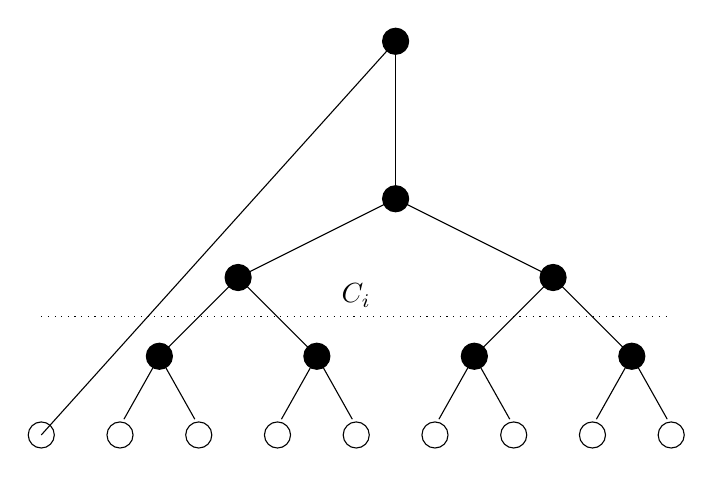
\begin{tikzpicture}
		\node[circle,draw] at (0,0) {};
		
		\node[circle,draw] at (1, 0){};
		\node[circle,draw,fill=black] at (1.5, 1){};
		\draw (1.5, 1) --(1.95, 0.2);
		\draw (1.5, 1) --(1.05, 0.2);
		\node[circle,draw] at (2,0) {};
		
		\node[circle,draw,fill=black] at (2.5, 2){};
		\draw (2.5, 2) --(1.5, 1);
		\draw (2.5, 2) --(3.5, 1);

		\node[circle,draw] at (3, 0){};
		\node[circle,draw,fill=black] at (3.5, 1){};
		\draw (3.5, 1) --(3.95, 0.2);
		\draw (3.5, 1) --(3.05, 0.2);
		\node[circle,draw] at (4,0) {};
		
		\node[circle,draw,fill=black] at (4.5, 3){};
		\draw (4.5, 3) --(2.5, 2);
		\draw (4.5, 3) --(6.5, 2);

		
		\node[circle,draw,fill=black] at (4.5, 5){};
		\draw (4.5, 5) --(4.5, 3);
		\draw (4.5, 5) --(0, 0);
		
		
		\node[circle,draw] at (5, 0){};
		\node[circle,draw,fill=black] at (5.5, 1){};
		\draw (5.5, 1) --(5.95, 0.2);
		\draw (5.5, 1) --(5.05, 0.2);
		\node[circle,draw] at (6,0) {};
		
		\node[circle,draw,fill=black] at (6.5, 2){};
		\draw (6.5, 2) --(5.5, 1);
		\draw (6.5, 2) --(7.5, 1);
		
		
		\node[circle,draw] at (7, 0){};
		\node[circle,draw,fill=black] at (7.5, 1){};
		\draw (7.5, 1) --(7.95, 0.2);
		\draw (7.5, 1) --(7.05, 0.2);
		\node[circle,draw] at (8, 0){};
		
		\draw[dotted] (0, 1.5) -- node[above] {$C_i$} (8, 1.5);
	\end{tikzpicture}
\caption{A hierarchical clustering tree of $n=9$ points. This tree contains the clustering $C_i$ described in the proof of Lemma \ref{lemma:treesOnX}.}
\label{fig:treeStructure}
\end{figure}
\end{proof}

\VCDimT*
\begin{proof}
Let $n$ be as defined in the statement of the theorem. Let $M^2 \subseteq \mc X^2$ be a set of size $> n^2$. Define $M := \{x: (x, y) \in M^2 \text{ or } (y, x) \in M^2\}$. We know that $|M| > n$. Using lemma \ref{lemma:treesOnX}, there exists a set of clusterings $\mc C = \{C_1, \ldots, C_{s'}\}$ of size $s' > \frac{n!}{\lfloor n/2 \rfloor! \enspace 2^{\lfloor n/2 \rfloor}} \ge s$ such that each $T_i \in \mc F$ contains atmost one $C_j \in \mc C$. Thus, there exists a clustering $C_j$ which is not captured by any $T_i \in \mc F$. Hence, $l_{\mc F}$ can't shatter any set of size $> n^2$.
\end{proof}

